\section{Grundlagen}
\subsection{Industrie 4.0}
\subsubsection{Künstliche Intelligenz im industriellen Kontext}
\subsubsection{RAMI 4.0}
Das Refernzarchitekturmodell Industrie 4.0 ist ein Leitfaden für die Industrie und dient als Hilfestellung um die digitale Transformation in einem Unternehmen systematisch umzusetzten.
Es soll helfen, die komplexen Anforderungen an die Industrie 4.0 für die Allgemeinheit verständlich zu machen.


\newpage
\subsection{Digitaler Zwilling}
Digitale Zwillinge im industriellen Kontext nehmen eine zunehmend zentralle Rolle ein und das Interesse ist in den letzten Jahren immer mehr gestiegen.
Erstmals wurde das Konzept von M. Grieves im Jahr 2003 in einer Präsentation zum Product Lifecycle Management vorgestellt \cite{DTGrieves}. 
Grieves definierte drei zentrale Komponenten, die zusammen das Informationsmodell des digitalen Zwilling bilden:
\begin{itemize}
    \item ein reales Objekt in der physischen Welt,
    \item ein digitales Abbild dieses Objekts in einem virtuellen Raum, sowie
    \item eine Schnittstelle, die den Informationsfluss zwischen diesen beiden ermöglicht.
\end{itemize}

Auf Basis des von Grieves entwickelten Informationsmodells hat sich der Begriff des digitalen Zwillings stetig weiter entwickelt und in verschiedenen Bereichen Einzug erhalten. 
Aufgrund der verschiedenen Fachgebiete und unkonsistentr Definitionen des digitalen Zwillings haben sich in der Vergangenheit unterschiedliche Ausprägungen des Begriffs des digitalen Zwillings gebildet.
Diese unterscheiden sich insbesondere in der Tiefe der Datenintegration zwischen dem physischen Objekt und seinem virtuellen Abbild.
Während ein einfacher digitaler Zwilling lediglich ein einfaches Modell mit statischen Daten ist, ermöglichen fortgeschrittene Zwillinge einen bidrektionalen Datenaustausch zwischen physischem und virtuellem Objekt. 

Grundsätzlich lassen sich digitale Zwilling nach Typ und Instanz unterscheiden.
Typen sind allgemeine Abbilder, die grundlegende Eigenschaften und Verhaltensmodelle einer Produktgruppe beschreiben. 
Sie können mit einer Klasse in der Softwarentwicklung verglichen werden, die als Vorlage für konkrete Instanzen dienen.
Typen können zum Beispiel einen bestimmten Maschinentyp hinsichtlich Aufbau, Stuktur oder Schnittstellen beschreiben, ohne dabei Bezug zu einer einzelnen physischen Maschine zu nehmen.
Instanzen wiederrum sind einzigartig, und beschreiben ein konkretes Produkt, wie zum Beispiel eine Maschine, die einzigartig über eine Seriennummer identifizierbar ist.
Häufig sind Instanzen Aussprägungen eines Types mit einer Verbindung zu einem realen Objekt, wodurch beispielsweise die Überwachung des Zustands einer Maschine ermöglicht wird.
Analog zur Softwarentwicklung können diese als instanziiertes Objekt einer Klasse gesehen werden. \cite{ZEISS}

Drei wesentliche Konzepte, die immmer wieder im Zusammenhang des digitalen Zwillings gleichbedeutend gennant werden sind das digitale Modell, der digitale Schatten und der digitale Zwilling. \cite{ClassificationDT}
Die Klassifizierung nach der Art des Informationsfluss ist hierbei nur für Instanzen des digitalen Zwillings sinnvoll.
Sie unterscheiden sich dabei wesentlich in der Art des Informationsflusses.
Digitale Modelle sind statische Abbilder physischer Objekte, haben jedoch keine Verbindung zu diesen. 
Oft werden sie zur Veranschauclichung oder Konstruktion genutzt, wie zum beispiel ein 3D-Modell einer Maschine.
Zwar können reale Daten, wie etwa Maße oder Materialeigenschaften einer Anlage oder Maschine in ein solches Modell integriert werden, allerdings erfolgt die Eingabe dabei immmer manuel.
Änderungen an dem realen Objekt werden nicht automatisch aktualisiert und bleiben somit ohne Einfluss auf das digitale Modell.
Der digitale Schatten ergänzt das digitale Modell um eine unindirektionale Verbindung zum realen Objekt.
Dabei fließen Daten des physischen Objekts meist in Echtzeit über zum Beispiel geeignete Sensoren zum digitalen Objekt.
Der Schatten bildet den aktuellen Zustand des Objekts ab, hat aber keine Rückkoplung zu diesem.
Ein typisches Beispiel für einen digitalen Schatten wäre das Condition Monitoring, wobei der Zustand einer Maschine mit geeigneten Sensoren abgebildet wird.
Mit einer aktiven Rückkoplung zum realen Objekt wird der digitale Schatten zum digitalen Zwilling.
Es entsteht eine Feedback-Schleife und erlaubt dem virtuellen Objekt Einfluss auf das reale System zu nehmen.

% Quelle: file:///C:/Users/Heinke/Documents/Bachelorarbeit/02%20Literatur/Digitaler_Zwilling/Klassifizierung_DT.pdf

\begin{figure}[htbp]
    \centering
    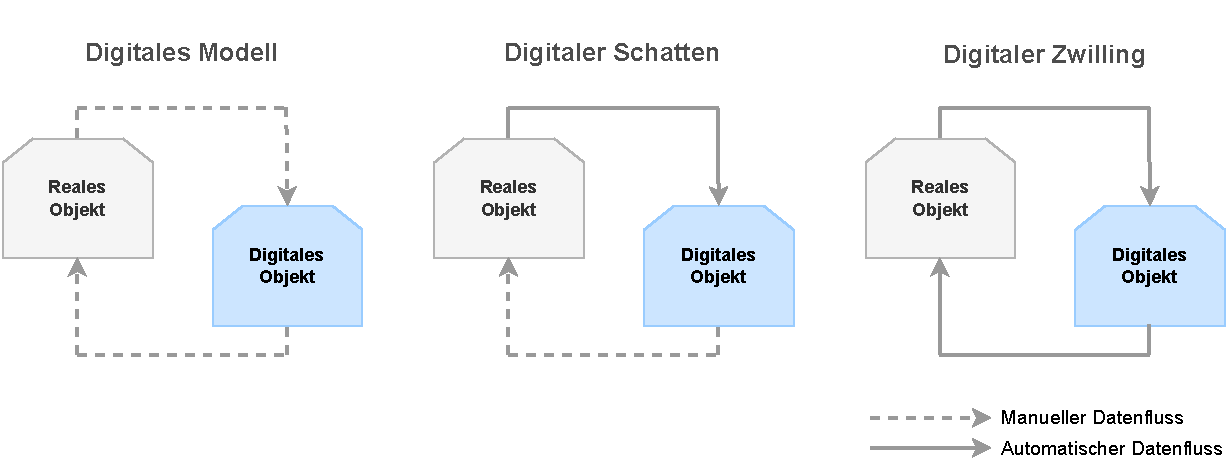
\includegraphics[width=1\textwidth]{Bilder/klassifizierung_DT.pdf}
    \caption{Klassifizierung des DT}
    \label{fig:klassifizierungDT}
\end{figure}

% Digitales Modell, digitaler Schatten und digitaler zwilling
Digitale Zwillinge werden im industriellen Umfeld in vielen unterschiedlichen Bereichen eingesetzt. 
Sie kommen entlang des gesamten Lebenszyklus eines Produkts oder Systems zum Einsatz - von der Entwicklung über die Produktion bis hin zum Betrieb und der Wartung. 
Bereits bei der Entwicklung von Produkten können digitale Zwillinge einen erheblichen Vorteil bieten. 
Indem bereits frühzeitig digitale Modelle oder Simulationen eingesetzt werden, entfällt die Notwendigkeit physischer Prototypen, was Entwicklungszeiten und Kosten deutlich senken kann. Während der Produktion ermöglichen sie eine durchgängige Überwachung, Analyse und Optimierung von Fertigungsprozessen durch die Integration von Echtzeitdaten.
Sie unterstützen die virtuelle Inbetriebnahme von Maschinen und dienen als Grundlage für die vorausschauende Wartung (Predictive Maintenance), wodurch Stillstandzeiten einer Maschine reduziert werden können.
Darüber hinaus können verschiedene Prozesse durch Simulation unter unterschiedlichen Bedingungen getestet und optimiert werden. 
Nicht zuletzt dienen digitale Zwillinge als zentrale Datenplattform, in der alle relevanten Informationen aus verschiedenen Datenquellen gebündelt werden.
Sie bilden somit eine konsistente Datenbasis und können beispielsweise bei dem Entwicklungsprozess eines Produktes helfen. \cite{DTForSmartManufacturing}

% Trotz der zahlreichen Vorteile gibt es auch einige Herausforderungen bei der Einführung digitaler Zwillinge in einem Unternehmen.
% Zunächst müssen Daten aus unterschiedlichsten Systemen wie ERP oder MES in ein digitales Modell zusammengefasst werden.
% Häufig liegen diese jedoch in heterogenen Formaten vor, was die Integration erheblich erschwert.


% Darüber hinaus gestaltet sich die Modellierung selbst oft als anspruchsvoll, da sowohl spezielles Fachwissen als auch geeignete Tools zur Modellierung benötigt werden.
% Insbesondere beim Einsatz digitaler Zwillinge über Unternehmensgrenzen hinweg muss ein einheitliches Verständnis der Daten geschaffen werden.
% Uneindeutige Beschreibungen können zu Fehlinterpretationen -und entscheidungen führen.
% Nicht zuletzt stell die Cybersicherheit eine zentrale Herausforderung dar - vor allem wenn cloudbasierte Lösungen oder unternehmensübergreifende Datenräume genutzt werden.


Herausforderungen.




% Definition nach Stark und Damerau des DT: 

% A digital twin is a digital representation of an active unique product (real device, object, machine, service, or intangible asset) or unique product-service system (a system consisting of a product and a related service) that comprises its selected characteristics, properties, conditions, and behaviors by means of models, information, and data within a single or even across multiple life cycle phases.

% \url{https://link.springer.com/referenceworkentry/10.1007/978-3-642-35950-7_16870-1#citeas}

\newpage
\subsection{Asset Administration Shell}
Die Asset Administration Shell (AAS) - deutsch Verwaltungsschale - ist eine Schlüsselkomponente innerhalb des Referenzarchitekturmodell Industrie 4.0 \cite{RAMI4.0} und bildet die Grundlage für die Umsetzung und Entwicklung interoperabler digitaler Zwillinge im industriellen Umfeld.
Sie wurde maßgeblich von der Plattform Industrie 4.0 entwickelt und erstmlas im Jahr 2016 als Teil von RAMI 4.0 vorgestellt.
Seit ihrer Einführung wurde die AAS kontinuierlich weiterenwtickelt und ist mittlerweile in der internationalen Norm IEC 63278-1:2023 \cite{AASIEC63278} standardisiert.
% Darin wird die AAS als "strukturierte, standardisierte digitale Repräsentation eines Assets" definiert.

Seit 2020 wird die Umsetzung und Weiterentwicklung der AAS von der Industrial Digital Twin Association (IDTA) organisiert und gesteuert.
Ziel der IDTA ist es, den digitalen Zwilling auf Basis der AAS zu standardisieren und in Form von Open Source Softwarelösungen in das industrielle Umfeld zu integrieren.
Die AAS wird dabei in mehreren Spezifikationen der IDTA dokumentiert und beschrieben.
Aktuell bildet die AAS Version 3 den neuesten Entwicklungsstand und ist ebenfalls die Basis für diese Arbeit.
% evtl die Quelle wenn gut https://www.zvei.org/themen/start-der-industrial-digital-twin-association-idta

Die AAS repräsentiert ein Asset digital, indem sie alle relevanten Daten, Eigenschaften und Funktionen über den gesamten Lebenszyklus hinweg in strukturierter und standardisierter Form bereitstellt. 
Sie fungiert somit als digitales Gegenstück eines realen Objekts - also als digitaler Zwilling.
Die Informationen sind in sogenannten Submodellen organisiert, die jeweils spezifische Aspekte eines Assets abbilden.
Dabei kann es sich sowohl um physische Assets (z.B. Maschinen, Anlagen) als auch um virtuelle Assets (z.B. Software, Konzepte) handeln. 
Eine AAS ist stets eindeutig einem Asset zugeordnet und global identifizierbar. 
Durch die Kombination eines Assets mit seiner AAS entsteht eine sogenannte Industrie-4.0-Komponente.

% Durch die standardisierte Struktur bildet die Verwaltungsschale die Grundlage für einen einheitlichen Informationsaustausch über System -und Unternehmensgrenzen hinweg.
% Verwaltungsschalen repräsentieren immer genau ein Asset und müssen global eindeutig identifizierbar sein.
% In der Industrie können Assets physische Objekte, wie eine Anlage oder eine Maschine sein oder aber auch virtuelle Elemente wie Software oder eine Idee.
% In RAMI 4.0 wird davon ausgegangen, das Assets immmer einen konkreten Nutzen für ein Unternehmen bzw. eine Organisation bieten.
\vspace{2em}
\begin{figure}[htbp]
    \centering
    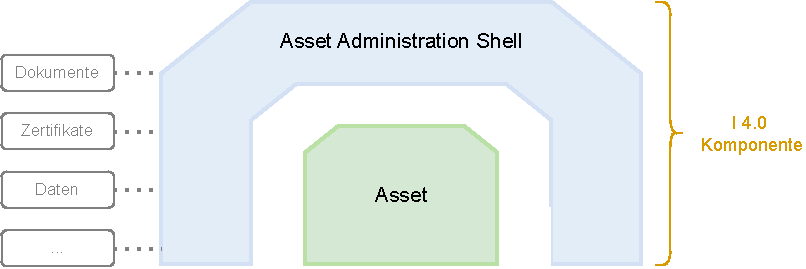
\includegraphics[width=1\textwidth]{Bilder/i4_komponente_neu.pdf}
    \caption{Industrie 4.0 Komponente}
    \label{fig:klassifizierungDT}
\end{figure}
Allgemein kann zwischen Typ -und Instanz-Verwaltungsschalen unterschieden werden.
Typ-AAS beschreiben allgemeine Eigenschaften eines Produkttypen oder einer Produktlasse wie einen bestimmten Maschinen-Typ, während Instanz-Verwaltungsschalen immer einem spezifischen Objekt zugeordnet werden.
Typen können zum Besipiel allgemeine Dokumente, Eigenschaften oder Merkmale enthalten, die für eine bestimmte Maschinenart gelten.
Sie dienen als standardisierte, wiederverwendbare Vorlage für das Erstellen von Instanzen.
Im Gegensatz dazu werden Instanzen immer einem konkreten physischen Objekt zugewiesen - etwa durch die Seriennummer, den aktuellen Standort oder den Betriebszustand einer Maschine.

Bestimmte Aspekte eines Assets werden in verschiedenen Submodellen verwaltet.
Man kann sich dies wie ein Schubladensystem vorstellen, wobei jede Schublade einen bestimmten Bereich des Assets abdeckt - beispielsweise die technischen Stammdaten, das Typenschild Wartungsinformationen oder Zustandswerte einer Maschine.
Die Auswahl der Submodelle hängt dabei immer von dem konkreten Asset ab, dass modelliert werden soll.
Genau wie die AAS müssen diese Teilmodelle global eindeutig identifizierbar sein.
Ein Submodell besteht dabei immmer aus verschiedenen Submodellelementen. Zu den Wichtigsten zählen:

\begin{itemize}
    \item \textbf{Property}: einfaches Merkmal mit bestimmten Datentyp, z.B. Name
    \item \textbf{Entity}: Eigenständiges Teilobjekt eines Assets, z.B. ein Bauteil 
    \item \textbf{File}: Eingebettete oder referenzierte Datei, z.B. CAD-Modell
    \item \textbf{ReferencElement}: Verweis auf anderes (externes) Element oder Objekt
    \item \textbf{RelationShipElement}: Beziehung verschiedener Elemente oder Assets
    \item \textbf{SubmodelElementCollection}: Sammlung von Submodellelementen
\end{itemize}

Es ist wichtig alle Submodelle bzw. alle Elemente über eine eindeutige Semantik zu beschreiben.
Hierfür gibt es sogenannte "Concept Desciptions". Diese enthalten unter anderem Beschreibugen, Definitionen, Einheiten und externe Referenzen für ein bestimmtes Element.
Sie helfen bei der Klassifizierung von Daten und sorgen für ein gemeinsames Verständnis unterschiedlicher Systeme.
Diese Beschreibungen können entweder direkt in die AAS eingebetet werden oder über externes Standards wie zum Beispiel ECLASS referenziert werden.
ECLASS basiert auf dem Datenmodell der Norm IEC 61360 [IEC 61360], welche eine standardisierte Struktur für Merkmale und deren semantische Beschreibung definiert.
Zur Veranschaulichung wird nachfolgend ein vereinfachtes Schema des Metamodells der Verwaltungsschale in Abbildung 3 dargestellt. \cite{SpezifikationPart1}

\begin{figure}[htbp]
    \centering
    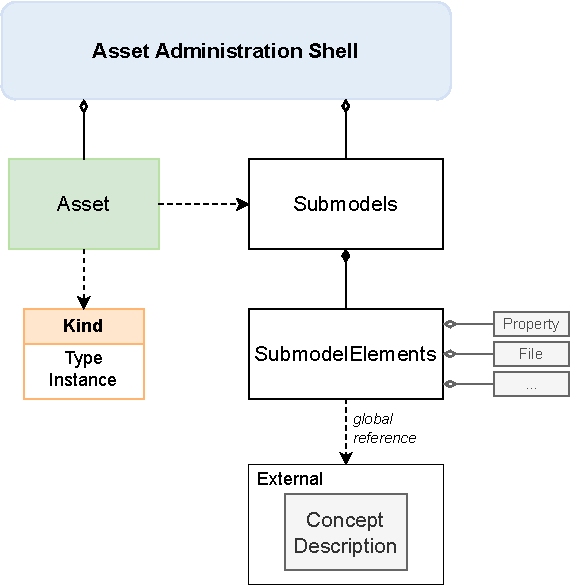
\includegraphics[width=0.7\textwidth]{Bilder/Metamodel.pdf}
    \caption{Metamodell der AAS}
    \label{fig:MetamodellAAS}
\end{figure}

Um die Erstlleung von Submodellen zu erleichtern und gleichzeitig Interoperabilität zu gewährleisten, stellt die IDTA standardisierte Submodellvorlagen - sogenannte Submodel Templates - zur Verfügung.
Aktuell sind 34 dieser Templates veröffentlicht, viele weitere sind in der Entwicklung oder im Überprüfungsprozess und werden in Zukunft ergänzt.
Die bereits verfügbaren Templates enthalten unteranderem Submodelle wie das digitale Typenschild oder den Carbon Footprint.
Alle Eigenschaften innerhalb dieser Vorlagen werden dabei in Verbindung mit dem ECLASS-Standard einheiltich semantisch beschrieben.
Diese Templates könen über ein zentrales Repository bezogen werden und bilden die Basis für eine interoperable semantische Datenstruktur.

Der Austausch von Informationen über die AAS kann auf unterschiedliche Weise erfolgen.
Die einfachste Möglichkeit ist der Austausch über Dateien. Hierfür gibt es speziell für die AAS entwickelte AASX-Dateien, die einen einfachen Austausch statischer Verwaltungsschalen (Typ 1) erlauben. \cite{SpezifikationPart5}
Hierbei werden alle Daten, Beziehungen, die Struktur sowie zugehörige Dateien der AAS serialisiert in ein AASX-ZIP-Dateiformat gespeichert. Die Datei kann schließlich über ein digitales Medium wie eine E-Mail oder eine Cloud-Plattform weitergegeben werden.  
Typ-2 Verwaltungsschalen hingegen werden von einer Laufzeitumgebung gehosted und ermöglichen dadurch einen dynamischen Zugriff auf Informationen. 
In der API Spezifikation werden drei Kernkomponenten beschrieben, die zusammen ein System für einen interoperablen, standardisierten Zugriff bilden. \cite{SpezifikationPart2}
Repositories speichern die Inhalte der AAS, einschließlich ihrer Submodelle und Concept Descriptions (siehe weiter unten).
Über definierte Schnittstellen (APIs) können Daten aus einer AAS oder einem Submodell gelesen oder geschrieben werden.
Der Zugriff kann dabei mit verschiedenen Technologien wie HTTP/REST, MQTT oder OPC UA stattfinden.
Registries dienen als zentraler Ort zur Registrierung von AAS und Submodellen anhand iherer eindeutigen IDs. Sie ermöglichen das Auffinden von AAS innerhalb eines Systems.
Discovery(-Server) unterstützen eine schnelle Suche, indem sie Beziehungen anhand verschiedener Schlüsselpaare speichern. So kann zum Beispeil eine AAS über eine Asset-ID gefunden werden. 
Die fortschrittlichste Form des Austauschs ist die Peer-to-peer Kommunikation, bei der I4.0-Komponenten (Typ 3-AAS) eigenständig über die I4.0-Sprache miteinander kommunizieren können.

\subsection{Digitaler Produktpass für Industrie 4.0}
Der \ac{dpp} ist ein zentrales Instrument der Europäischen Union zur Umsetzung einer nachhaltigen, digitalen Transformation.
Ziel ist es, die Transparenz über ökologische Merkmale von Produkten wie verwendete Materialien, Recylcebarkeit oder die CO2-Bilanz deutlich zu verbessern.
Hierzu müssen produktspezifische Daten über den gesamten Lebenszyklus hinweg aufgezeichnet und in einem menschen -und maschinenlesbarem Format bereitgestellt werden.
Langfristig soll dies zu einer Kreislaufwirtschaft und digitalen Wirtschaft innerhalb der EU führen.

Das Konzept des digitalen Produktpasse wurde erstmals im Rahmen des European Green Deal von der Europäischen Kommission im Jahr 2019 vorgestellt [Quelle: https://eur-lex.europa.eu/legal-content/EN/TXT/?uri=CELEX:52019DC0640].
Im Zuge der Ökodesign-Verordnugng (Eco Design for Sustainable Products Regulation (ESPR) ) [Quelle] wird der \acs{dpp} aktuell als verpflichtendes Mittel für zahlreiche Produktgruppen eingeführt.
Als erstes konkrete Anwendung wird der digitale Produktpass erstmals im Jahr 2027 für Batterien verpflichtend, wie in der EU-Batterieverordnung festgelegt.
Weitere Produktkategorien, darunter auch die Elektroindustrie und der Maschinen -und Anlagenbau werden in den nächsten Jahren folgen.

Die Bereitstellung der digitalen Produktpässe erfolgt gemäß den Anforderungen der ESPR in elektronischer Form. Dabei müssen diese untereinander interoperabel miteinander kommunizieren können.
Daten innerhalb eines Passes müssen standardisiert und strukturiert in einem menschen -und maschinenlesbarem Format zur Verfügung gestellt werden.
Je nach Art der Information werden verschiedene Zugriffsrechte für unterschiedliche Interessengruppen eingeführt. Damit soll der Schutz von geistigem Eigentum sichergestellt werden.
Verwaltet werden sollen die Daten dabei über einen zentralen Server bzw. ein Registry, in dem die verschiedenen \acsp{dpp} gespeichert bzw. zumindest registriert werden.
Der Zugriff auf konkrete Pässe soll möglichst einfach sein. Hierzu können zum Beispiel QR-Codes eingesetzte werden, die direkt am Produkt angebracht sind, und direkt zum \acs{dpp} führen.
Dafür ist es wichtig, das jedes Produkt global eindeutig über eine einzigartige Kennung beschrieben wird.
Quelle: vgl. https://cirpassproject.eu/wp-content/uploads/2023/03/ESPR-short-summary-Final.pdf

Während die regulatorischen Rahmenbedingungen schon mehr oder weniger final ausgearbeitet sind, bleibt noch die Frage der konkreten technologischen Umsetzung.
Eine dezentrale Lösung zur Umsetzung bildet der von der ZVEI vorgestellte digitale Produktpass für die Industrie 4.0 (DPP 4.0). [DPP 4.0: An Architecture Proposal for a DPP-System to implement the EU Digital Product Passport for Industrial Products]
Der DPP 4.0 basiert dabei auf zwei etablierten Standards. Zum Einen das digitale Typenschild, und zum Anderen die Asset Administration Shell [Link zu Kapitel AAS].
Das digitale Typenschild ermöglicht - gemäß der Norm IEC 61406 [Quellle Norm] - die eindeutige Identifikation von Produkten über eine einzigartige Asset-ID.
Typischerweise wird diese in Form eines maschinenlesbarem Links oder QR-Codes an ein Produkt angebracht, wodurch ein direkter Zugriff auf den jeweiligen \acs{dpp} ermöglicht wird.

Das Konzept des DPP 4.0 sieht vor, dass Unternehmen ihre Produktpässe dezentral in einem eigenen Repository verwalten.
Dies soll Unternehmen helfen, Daten innerhalb eines Produktpasse bei Bedarf selbstständig zu aktualisieren.
Organisiert werden die Daten in verschiedenen Submodellen der Verwaltungsschale. 
Standardisierte Teilmodelle wie das digitale Typenschild, Dokumentationen oder der Product Carbon Footprint (PCF) helfen bei der Umsetzung der im \acs{dpp} geforderten Daten.
Darüber hinaus können auch zusätzliche, nicht verpflichtende Informationen integrierte werden, sofern sie für bestimmte Stakeholder einen Mehrwert bieten.
Der Zugriff auf die Daten erfolgt über ein webbasiertes Portal. Verschiedene Interessengruppen erhalten dabei unterschiedliche Zugangsrechte. 
Hierfür werden bestimmmte Teilmodelle für unterschiedliche Gruppen freigegeben.
Eine schemantische Darstellung des DPP 4.0 ist in Abbildung xy dargestellt.

\begin{figure}[htbp]
    \centering
    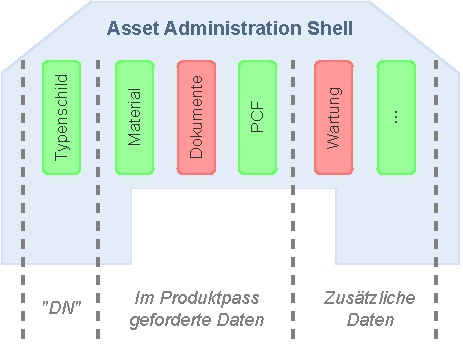
\includegraphics[width=0.7\textwidth]{Bilder/dpp_konzept.pdf}
    \caption{Konzept des DPP 4.0}
    \label{fig:klassifizierungDT}
\end{figure}


Exemplarisch gezeigt wird dies in einem PCF Showcase...
Ein Zwei abschließende Worte...


%

\subsection{robocell Füll -und Verschließmodul}

Was ist die robocell? Wodurch zeichnet sie sich aus?

Eingehen auf das Füllmodul


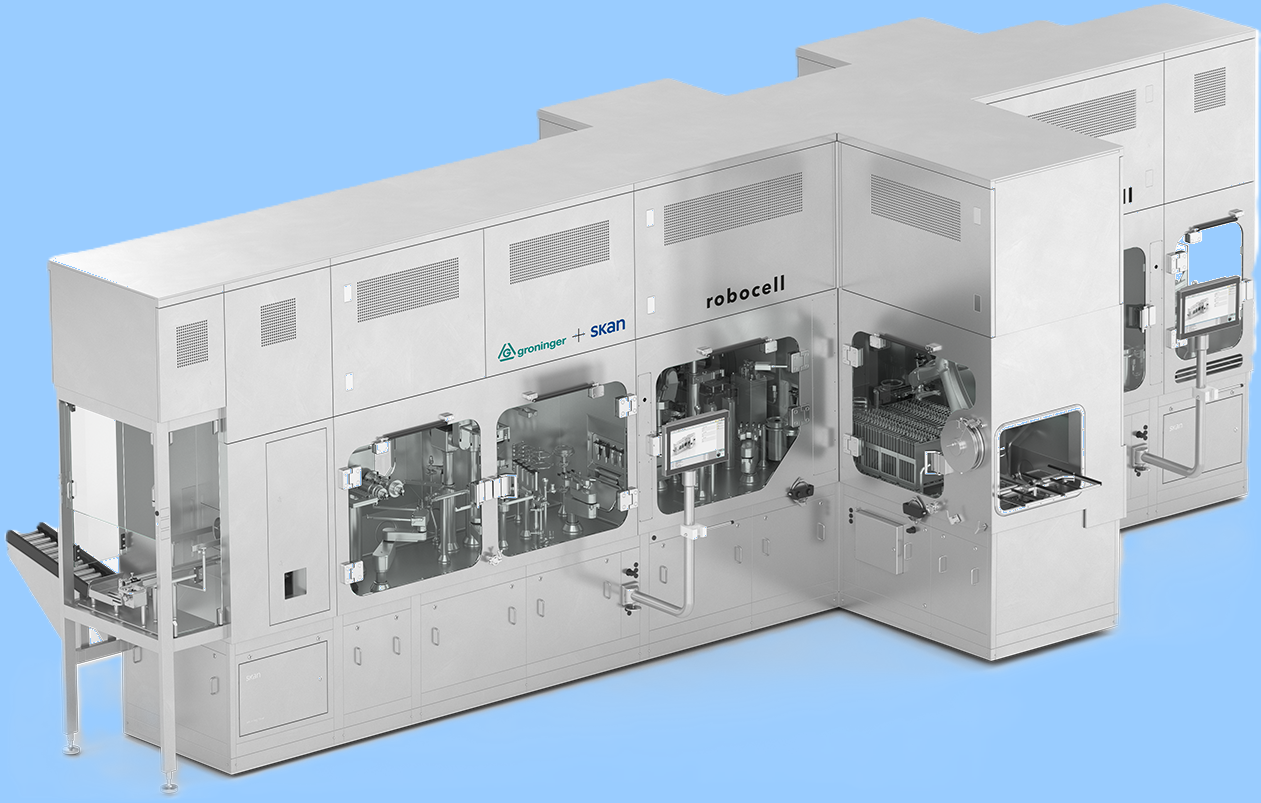
\includegraphics{Bilder/robocell_FS2_rgb_Logo.png}
\subsection{Technologische Grundlagen}
Brauche ich das?
\subsubsection{AASX Package Exlporer}
Der von Michael Hoffmeister entwickelte AASX Package Explorer ist ein Toll/Anwendung zur manuellen Errstellung von Verwaltungschalen.
Er ermöglicht das Modellieren von Verwaltungsschalen mit allen Elementen dieser.
Hiermit können ganze Verwaltungsschale erstellt werden und in eine Datei wie eine aasx Datei oder XML Datei geschrieben werden.
Er bringt alles mit, was für die Erstellung von Verwaltungsschalen benötigt wird.
Man kann AAS anschauen und bearbeiten.
AUch kann ein Server angebunden werden.
\subsubsection{OPC UA}
\subsubsection{Eclipse BaSyx }
BaSyx ist eine von der EClipse Foundation entwickelte Softwarelösung für die Erstellung und Verwaltung von Asset Administration Shells.
Die Architektur von BaSyx basiert auf einer Vielzahl verschiedener Off-The-Shelf-Komponenten, die alle als Docker Container frei zugänglich sind und somit einfach in eine bestehende Umgebung integriert werden können. 
Die Kernkomponenten sind:

\begin{itemize}
    \item aas-registry: Ermöglicht die Registrierung und Verwaltung von Verwaltungsschalen
    \item sm-registry: Ermöglicht die Registrierung und Verwaltung von Submodellen
    \item aas-env: Enthält Repositorys für AAS, Submodelle und Concept Descriptions
    \item aas-ui: Weboberfläche zur Visualisierung und Bearbeitung von Verwaltungsschalen
\end{itemize}

Durch die Kombination der verschiedenen Komponenten bietet BaSyx eine vollständige Laufzeitumgebung für die Verwaltung und Interaktion von digitalen Zwillingen auf Basis der Verwaltungsschale.



